\documentclass[fsharpNotes.tex]{subfiles}
\graphicspath{ {./figures/} }

\begin{document}
\chapter{Making programs and documenting them}

\abstract{
  Introductory text about the objectivs of this chapter
  \begin{itemize}
  \item \dots
  \end{itemize}
}

\section{7 step guide to making programs}
\dots

\section{Programming as a commication activity}
\label{chap:documentation}
Documentation is a very important part of writing programs, since it is most unlikely that you will be writing really obvious code. Moreover, what seems obvious at the point of writing may be mystifying months later to the author and to others. Documentation serves several purposes:
\begin{enumerate}
\item Communicate what the code should be doing.
\item Highlight big insights essential for the code.
\item Highlight possible conflicts and/or areas where the code could be changed later.
\end{enumerate}
The essential point is that coding is a journey in problem-solving, and proper documentation is an aid in understanding the solution and the journey that lead to it. Documentation is most often a mixture of in-code documentation and accompanying documents. Here, we will focus on in-code documentation which arguably causes problems in multi-language environments and run the risk of bloating code.

F\# has two different syntaxes for comments. Comments can be block
comments: \jon{color of '*' is wrong.}
%
\begin{verbatimwrite}{\ebnf/blockComment.ebnf}
(**<*any text*>**)
\end{verbatimwrite}
\syntax{\ebnf/blockComment.ebnf}{Block comments.\idxss{(**)@\lstinline{(**)}}}
%
The comment text \lstinline[language=syntax]{(*<*any text*>*)} can be any text and is stilled parsed by F\# as keywords and basic types, implying that \lstinline!(* a comment (* in a comment *) *)! and \lstinline[morecomment={[l][\color{commentsColor}]{(*}}]!(* "*)" *)! are valid comments, while \lstinline!(* " *)! is invalid.

Alternatively, comments may also be line comments,
%
\begin{verbatimwrite}{\ebnf/lineComment.ebnf}
//<*any text*>
\end{verbatimwrite}
\syntax{\ebnf/lineComment.ebnf}{Line comments.\idxss{//@\lstinline{//}}}
%
where the comment text ends after the first newline.

The F\# compiler has an option for generating \idx{Extensible Markup Language} (\idx{XML}) files from scripts using the C\# documentation comments tags\footnote{For specification of C\# documentations comments see ECMA-334: \url{http://www.ecma-international.org/publications/files/ECMA-ST/Ecma-334.pdf}}. The XML documentation starts with a triple-slash \lstinline{///}, i.e., a lineComment and a slash, which serve as comments for the code construct that follows immediately after. XML consists of tags which always appear in pairs, e.g., the tag ``tag'' would look like \lstinline[language=xml]!<tag> ... </tag>!. F\# accept any tags, but recommends those listed in \Cref{tab:xmlTags}.
\begin{table}
  \centering
  \rowcolors{2}{oddRowColor}{evenRowColor}
  \begin{tabularx}{\linewidth}{|l|X|}
       \hline
    \rowcolor{headerRowColor} Tag & Description\\
    \hline
    \lstinline[language=xml]!<c>! &Set text in a code-font.\\
    \hline
    \lstinline[language=xml]!<code>! &Set one or more lines in code-font.\\
    \hline
    \lstinline[language=xml]!<example>! &Set as an example.\\
    \hline
    \lstinline[language=xml]!<exception>! &Describe the exceptions a function can throw.\\
    \hline
    \lstinline[language=xml]!<list>! &Create a list or table.\\
    \hline
    \lstinline[language=xml]!<para>! &Set text as a paragraph.\\
    \hline
    \lstinline[language=xml]!<param>! &Describe a parameter for a function or constructor.\\
    \hline
    \lstinline[language=xml]!<paramref>! &Identify that a word is a parameter name.\\
    \hline
    \lstinline[language=xml]!<permission>! &Document the accessibility of a member.\\
    \hline
    \lstinline[language=xml]!<remarks>! &Further describe a function.\\
    \hline
    \lstinline[language=xml]!<returns>! &Describe the return value of a function.\\
    \hline
    \lstinline[language=xml]!<see>! &Set as link to other functions.\\
    \hline
    \lstinline[language=xml]!<seealso>! &Generate a See Also entry.\\
    \hline
    \lstinline[language=xml]!<summary>! &Main description of a function or value.\\
    \hline
    \lstinline[language=xml]!<typeparam>! &Describe a type parameter for a generic type or method.\\
    \hline
    \lstinline[language=xml]!<typeparamref>! &Identify that a word is a type parameter name.\\
    \hline
    \lstinline[language=xml]!<value>! &Describe a value.\\
    \hline
  \end{tabularx}
  \caption{Recommended XML tags for documentation comments, from ECMA-334 3rd Edition, Annex E, Section 2.}
  \label{tab:xmlTags}
\end{table}
If no tags are used, then it is automatically assumed to be a \lstinline[language=xml]!<summary>!. An example of a documented script is shown in \Cref{commentExample}.
is:
%
\fsCode{commentExample}{commentExample}{Code with XML comments.}{}
%

Mono's \lstinline[language=console]{fsharpc} command may be used to extract the comments into an XML file, as demonstrated in \Cref{convertingToXML}.
\begin{codeNOutput}[label=convertingToXML]{, Converting in-code comments to XML.}
  \begin{lstlisting}[language=console]
$ fsharpc --doc:commentExample.xml commentExample.fsx 
F# Compiler for F# 4.0 (Open Source Edition)
Freely distributed under the Apache 2.0 Open Source License
\end{lstlisting}
% $
\end{codeNOutput}
This results in an XML file with the content shown in \Cref{XMLExample}.
\begin{codeNOutput}[label=XMLExample]{, An XML file generated by \lstinline[language=console]{fsharpc}.}
  \lstinputlisting[language=xml, numbers=left, numbersep=6pt, numberstyle=\scriptsize\color{white}, breakatwhitespace=false]{src/commentExample.xml}
\end{codeNOutput}
The extracted XML is written in C\# type by convention, since F\# is part of the Mono and .Net framework that may be used by any of the languages using Assemblies. Besides the XML inserted in the script, the XML has added the \lstinline[language=xml]!<?xml ...>! header, \lstinline[language=xml]!<doc>!, \lstinline[language=xml]!<assembly>!, \lstinline[language=xml]!<members>!, and \lstinline[language=xml]!<member>! tags. The header and the  \lstinline[language=xml]!<doc>! tag are standards for XML. The extracted XML is geared towards documenting big libraries of codes and thus highlights the structured programming organisation, see \Cref{chap:modules,chap:oop}, and \lstinline[language=xml]!<assembly>!, \lstinline[language=xml]!<members>!, and \lstinline[language=xml]!<member>! are indications for where the functions belong in the hierarchy. As an example, the prefix \lstinline[language=xml]!M:CommentExample.! indicates that the method is in the namespace \lstinline{commentExample}, which in this case is the name of the file. Furthermore, the function type
\begin{quote}
  \lstinline!val solution : a:float->b:float->c:float->sgn:float->float!
\end{quote}
is in the XML documentation
\begin{quote}
  \lstinline[language=xml,basicstyle=\footnotesize]!M:CommentExample.solution(System.Double,System.Double,System.Double,System.Double)!,
\end{quote}
which is the C\# equivalent.

An accompanying program in the Mono suite is \lstinline[language=console]!mdoc!, whose primary use is to perform a syntax analysis of an assembly and generate a scaffold XML structure for an accompanying document. With the \lstinline[language=console]!-i! flag, it is further possible to include the in-code comments as initial descriptions in the XML. The XML may be updated gracefully by \lstinline[language=console]!mdoc! as the code develops, without destroying manually entered documentation in the accompanying documentation. Finally, the XML may be exported to HTML.

The primary use of the \lstinline[language=console]{mdoc} command is to analyze compiled code and generate an empty XML structure with placeholders to describe functions, values, and variables. This structure can be updated and edited as the program develops, and the edited XML files can be exported to \idx{Hyper Text Markup Language} (\idx{HTML}) files and viewed in any browser. Using the console, all of this is accomplished by the procedure shown in \Cref{XMLToHTML}, and the result is shown in \Cref{fig:htmlDocumentExample}.
\begin{codeNOutput}[label=XMLToHTML]{, Converting an XML file to HTML.}
\begin{lstlisting}[language=console]
$ mdoc update -o commentExample -i commentExample.xml commentExample.exe 
New Type: CommentExample
Member Added: public static double determinant (double a, double b, double c);
Member Added: public static double solution (double a, double b, double c, double sgn);
Member Added: public static double a { get; }
Member Added: public static double b { get; }
Member Added: public static double c { get; }
Member Added: public static double xp { get; }
Namespace Directory Created: 
New Namespace File: 
Members Added: 6, Members Deleted: 0
$ mdoc export-html -out commentExampleHTML commentExample
.CommentExample
\end{lstlisting}
\end{codeNOutput}
\begin{figure}
  \centering
  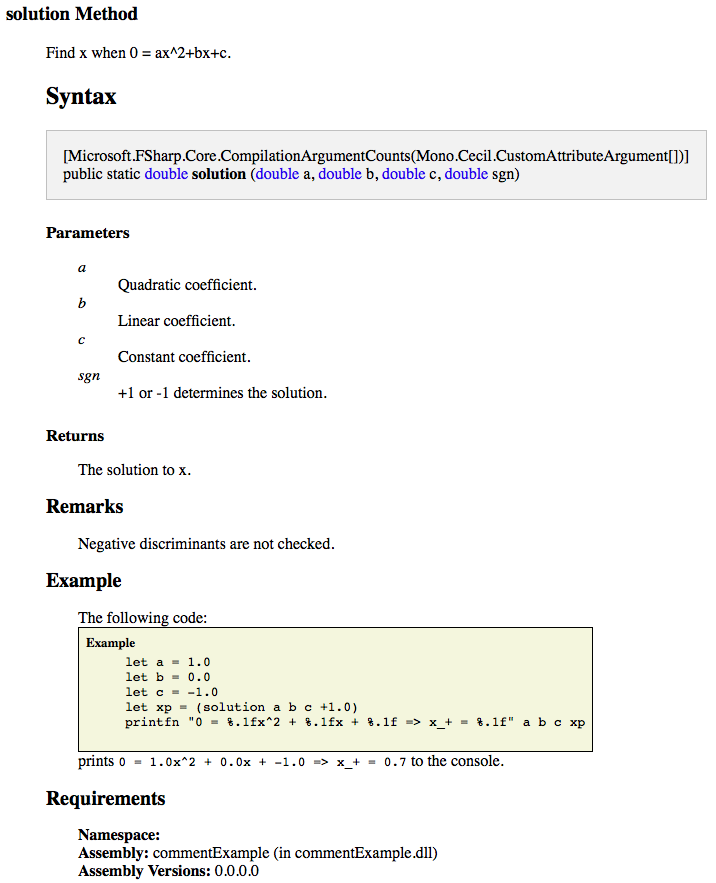
\includegraphics[width=\linewidth]{mdocOutput}
  \caption{Part of the HTML documentation as produced by \lstinline[language=console]{mdoc} and viewed in a browser.}
  \label{fig:htmlDocumentExample}
\end{figure}
A full description of how to use \lstinline[language=console]{mdoc} is found here\footnote{\url{http://www.mono-project.com/docs/tools+libraries/tools/monodoc/generating-documentation/}}.

\section{Key concepts and terms in this chapter}
Summary text about the key concepts from this chapter
\begin{itemize}
\item \ldots
\end{itemize}
\end{document}

